\documentclass[
a4paper,                        % paper size
11pt,                           % font size
twoside,                        % two sided
footsepline,                    % add a line to separate the footer
headsepline,                    % add a line to separate the header
headexclude,                    % header does not belong to the text
footexclude,                    % footer does not belong to the text
pagesize,                       % set the pagesize in a DVI document
bibtotocnumbered,               % add the bibliography to the TOC
idxtotoc                        % add the index to the TOC
%openright,                      % start a new chapter on the right page
%,DIV12
%,draft
]{scrreprt}

\usepackage{nameref}            % nameref, varioref, hyperref must be
                                % used in this order (see hyperref
                                % README)!
\usepackage[draft]{varioref}    % defines \vref
\usepackage{hyperref}           % automatically creates links when
                                % using pdflatex, defines \url
\usepackage{ifpdf}              % defines \ifpdf
\usepackage{graphicx}           % handles graphics
\usepackage{makeidx}            % creates the index
\usepackage{fancybox}

%%%%%%%%%%%%%%%%%%%%%%%%%%%%%%%%%%%%%%%%%%%%%%%%%%
%%%%%%%%%%%%%%%%%%%%%%%%%%%%%%%%%%%%%%%%%%%%%%%%%%
%%%%%%%%% New Commands and Environments %%%%%%%%%%
%%%%%%%%%%%%%%%%%%%%%%%%%%%%%%%%%%%%%%%%%%%%%%%%%%
%%%%%%%%%%%%%%%%%%%%%%%%%%%%%%%%%%%%%%%%%%%%%%%%%%
\newcommand{\es}{\textsf{ESPResSo}}
\newcommand{\ie}{\textit{i.e.\/}}
\newcommand{\eg}{\textit{e.g.\/}}
\newcommand{\etal}{\textit{et al.\/}}

\newcommand{\variant}[2]{(#1) \texttt{#2}\\}
%\newcommand{\lit}[1]{\texttt{#1}}
\newcommand{\var}[1]{\textrm{\textit{#1}}}
\newenvironment{syntax}{%
  \begin{Sbox}
    \begin{minipage}{0.9\linewidth}
    }{%
    \end{minipage}
  \end{Sbox}
  \begin{center}
    \fbox{\TheSbox}
  \end{center}
}

%%%%%%%%%%%%%%%%%%%%%%%%%%%%%%%%%%%%%%%%%%%%%%%%%%
%%%%%%%%%%%%%%%%%%%%%%%%%%%%%%%%%%%%%%%%%%%%%%%%%%
%%%%%%%%%%%%%%%% Other Settings %%%%%%%%%%%%%%%%%%
%%%%%%%%%%%%%%%%%%%%%%%%%%%%%%%%%%%%%%%%%%%%%%%%%%
%%%%%%%%%%%%%%%%%%%%%%%%%%%%%%%%%%%%%%%%%%%%%%%%%%
\pagestyle{headings}
\makeindex

%%%%%%%%%%%%%%%%%%%%%%%%%%%%%%%%%%%%%%%%%%%%%%%%%%
%%%%%%%%%%%%%%%%%%%%%%%%%%%%%%%%%%%%%%%%%%%%%%%%%%
%%%%%%%%%%%%%%%%% Main Document %%%%%%%%%%%%%%%%%%
%%%%%%%%%%%%%%%%%%%%%%%%%%%%%%%%%%%%%%%%%%%%%%%%%%
%%%%%%%%%%%%%%%%%%%%%%%%%%%%%%%%%%%%%%%%%%%%%%%%%%
\begin{document}
\titlehead{
  \begin{center}
    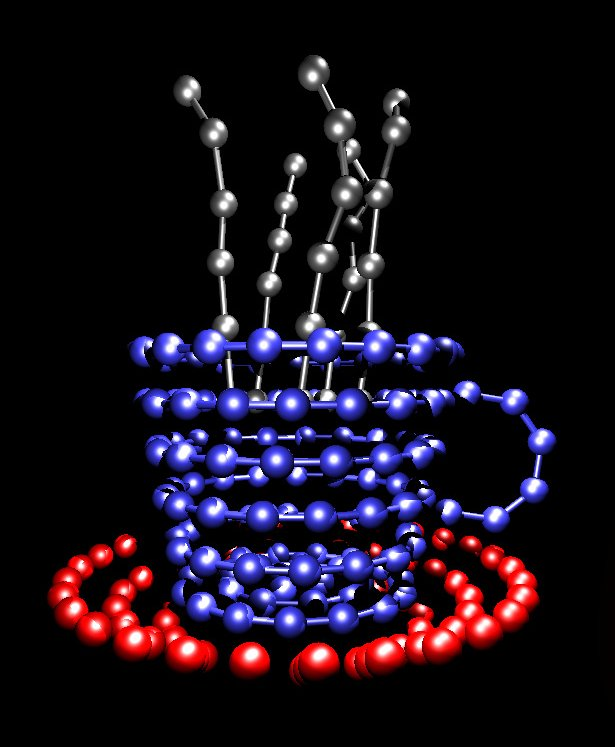
\includegraphics[width=5cm]{logo.jpg}
  \end{center}
}
%\subject{Dissertation}
\title{\es{} User's Guide}
%\author{Dipl.-Inform. Olaf~Lenz}
%\date{\today}
\maketitle

\tableofcontents

\chapter{Introduction}
\label{chap:intro}

(new)

\begin{itemize}
\item \es{} is a generic soft matter simulation packages
\item for molecular dynamics simulations in soft matter research
\item focussed on coarse-grained models
\item employs modern algorithms (Lattice-Boltzmann, DPD, P3M, \ldots)
\item written in C for maximal portability
\item Tcl-controlled
\item parallelized
\end{itemize}

\section{Guiding principles}
\label{sec:ideas}

(from paper: 2.1 Goals and principles)

\es
\begin{itemize}
\item does \emph{not} do the physics for you!
\item requires you to understand what you do (can not be used as a
  black box)
\item gives you maximal freedom (flexibility)
\item is extensible
\item integrates system setup, simulation and analysis, as this can't
  be strictly separated in soft matter simulations
\item has no predefined units
\item sets as few defaults as possible
\end{itemize}

\section{Algorithms contained in \es}

The following algorithms are implemented in \es{}:

\begin{itemize}
\item ensembles: NVE, NVT, NpT
\item charged systems:
  \begin{itemize}
  \item P3M for fully periodic systems
  \item ELC and MMM-family of algorithms for charged systems with
    non-periodic boundary conditions
  \item Maggs algorithm 
  \end{itemize}
\item Hydrodynamics:
  \begin{itemize}
  \item DPD (as a thermostat)
  \item Lattice-Boltzmann
  \end{itemize}
\end{itemize}

\section{Basic program structure}
\label{sec:structure}

(from paper: 2.2 Basic program structure)

\begin{itemize}
\item Control level: \texttt{Tcl}
\item ``Kernel'' written in \texttt{C}
\item This manual will focus on the control level
\end{itemize}

\section{On units}
\label{sec:units}

(new)

\begin{itemize}
\item Reduced units
\item comparison to ``real units''
\item three examples on different length scales
  \begin{itemize}
  \item some atomistic model?
  \item coarse-grained model (\eg lipid bilayer)
  \item billards?
  \end{itemize}
\end{itemize}

\chapter{Compiling and installing \es}
\label{chap:install}
\index{Installation|textbf}

\begin{itemize}
\item Compiling \es{} is a necessary evil
\item Features can be compiled in or not
\item For maximal efficiency, compile in only the features that you
  use
\item \es{} can be obtained from the \es{} home page
  \footnote{\url{http://www.espresso.mpg.de}}.
\item If you are looking for the \es binary or the object files, read
  \vref{sec:builddir}
\item other than in most packages, \es will probably not be installed,
  or it will only be installed locally. Refer to \vref{sec:installdir}
  for details.
\end{itemize}

\section{Source and build directories}
\label{sec:builddir}
\index{build directory} \index{source directory}

Usually, when a program is compiled, the resulting binary files are
put into the same directory as the sources of the program. In \es, the
\emph{source directory} that contains all the source files is
completely separated from the \emph{build directory} where the files
created by the build process are put. As the source directory is not
modified during the compilation process, it is possible to compile more
than one binary versions of \es from a single set of source files.

The location of the build directory is determined when
\texttt{configure} is called.  Depending on whether it is called from
the source directory where it resides, or from some other directory,
the build system will act different.

When \texttt{configure} is called from another current working
directory than the source directory, this directory will become the
\emph{build directory}.  All files will be generated below the build
directory.  This way, you can make as many builds of \es as you like,
each build having different compiler flags and built-in features, and
for as many platforms as you want.  All further commands concerning
compiling and running \es{} have to be called from this directory,
instead of from the source directory.

When \texttt{configure} is called from the source directory where the
script resides, the \es build system has limited built-in capabilities
to handle different computer hardware.  A new subdirectory is created
in the source directory and \texttt{configure} is recursively called
from this directory, making the subdirectory the build directory.  The
directory is called \texttt{obj-}\textit{platform}\texttt{/}, where
\textit{platform} is an automatically determined descriptor of the CPU
type where the script was started, \eg
\mbox{\texttt{obj-Athlon\_64-pc-linux}}.  Note that this heuristic
will work in many cases, but it may not always work as intended.  When
you notice any problems, you can always call \texttt{configure} from
another directory.

In this case it is also possible to run the commands \texttt{make} and
\texttt{Espresso} directly in the source directory.  Furthermore, the
option \texttt{--enable-chooser} will be set in the recursive call of
\texttt{configure} that activates the automatic binary chooser (see
section \vref{sec:installdir}).

\paragraph{Example}
When the source directory is \texttt{\$srcdir} (\ie{} the files where
unpacked to this directory), then the build directory can be set to
\texttt{\$builddir} by calling the \texttt{configure}-script from
there:
\begin{code}
cd $builddir
$srcdir/configure
make
Espresso
\end{code}

\section{\texttt{myconfig.h}: Activating and deactivating features}
\label{sec:myconfig}

\index{features} \index{myconfig.h} \index{configuration header} \es
has a large number of features that can be compiled into the binary.
However, it is not recommended to actually compile in all possible
features, as this will negatively affect \es's performance.  Instead,
compile in only the features that are actually required.  For the
developers, it is also possible to turn on or off a number of
debugging messages.  The features and debug messages can be controlled
via a configuration header file that contains C-preprocessor
declarations. Appendix \vref{chap:features} lists and describes all
available features.  When no configuration header is provided by the
user, a default header will be used that turns on the default
features.  The file \texttt{myconfig-sample.h} in the source directory
contains a list of all possible features that can be copied into your
own configuration file.

When you distinguish between the build and the source directory (see
\vref{sec:builddir}), the configuration header can be put in either of
these. Note, however, that when a configuration header is found in
both directories, the one in the build directory will be used.  For an
example how this can be employed, see section \ref{sec:builddir}.

By default, the configuration header is called \texttt{myconfig.h}.
The name of the configuration header can be changed either when the
\texttt{configure}-script is called with the option
\mbox{\texttt{--with-myconfig}} (see section \vref{sec:configure}), or
when \texttt{make} is called with the setting
\mbox{\texttt{myconfig=}\textit{myconfig\_header}} (see section
\vref{sec:make}).

The configuration header can be used to compile different binary
versions of \es with a different set of features from the same source
directory.  Suppose that you have a source directory \texttt{\$srcdir}
and two build directories \texttt{\$builddir1} and
\texttt{\$builddir2} that contain different configuration headers:

\begin{itemize}
\item \texttt{\$builddir1/myconfig.h}:
\begin{code}
#define ELECTROSTATICS
#define LENNARD-JONES
\end{code}

\item \texttt{\$builddir2/myconfig.h}:
\begin{code}
#define LJCOS
\end{code}
\end{itemize}

\noindent Then you can simply compile two different versions of \es via
\begin{code}
cd $builddir1
$srcdir/configure
make

cd $builddir2
$srcdir/configure
make
\end{code}


\section{Running \texttt{configure}}
\label{sec:configure}

% Description of basic options: --prefix, --exec-prefix, CPPFLAGS,
% CFLAGS, LDFLAGS

\index{configure} The shell script \texttt{configure} collects all the
information required by the compilation process. It will determine how
to use and where to find the different libraries and tools required by
the compilation process, and it will test what compiler flags are to
be used.  The script will find out most of these things automatically.
If something is missing, it will complain and give hints how to solve
the problem.  The generic syntax of calling the \texttt{configure}
script is:
\begin{code}
configure [\var{options} ...] [\var{variable}=\var{value} ...]
\end{code}

\noindent Note that in the \es build system, the files generated by
the configuration and compilation process are not placed next to the
source files, but into a separate \emph{build directory} instead.
Refer to section \vref{sec:builddir} for details.

\index{configure options} The behaviour of \texttt{configure} can be
controlled by the means of command line options. In the following,
only those command line options that are specific to \es will be
explained.  For a complete list of options and explanations thereof,
call
\begin{code}
configure --help
\end{code}

\subsection{Options}

\begin{description}
\item [\texttt{--enable-chooser}] This option will enable the
  automatic binary chooser mechanism for \es (see section
  \vref{sec:installdir}).  This option will be automatically enabled,
  when the \texttt{configure} script is called from the source
  directory, otherwise it will be disabled. It is not recommended to
  set the option manually.
\item[\texttt{--enable-debug}] This option will enable compiler flags
  required for debugging the \es binary and is disabled by default.
\item[\texttt{--enable-profiling}] This option will enable compiler
  flags required for profiling the \es binary and is disabled by
  default.
\item[\texttt{--disable-processor-optimization}] This option will
  control whether \texttt{configure} will check for several
  optimization flags to be used by the compiler. This option is
  enabled by default.
\item[\texttt{--disable-xlc-qipa}] This option is only useful when the
  IBM C-compiler \texttt{xlc} is used and will control whether or not
  the compiler flag \texttt{-qipa} is used.  If you come upon problems
  when using the \es binary on IBM machines, try using
  \texttt{--disable-xlc-ipa}. The option is enabled by default.
\item[\texttt{--with-myconfig=MYCONFIG\_HEADER}] This option sets the
  name of the local configuration header (see \vref{sec:myconfig}). It
  defaults to ``\texttt{myconfig.h}''.
\item[\texttt{--with-mpi=MPI}/ \texttt{--without-mpi}] Sets the MPI
  implementation that should be used, or disables MPI. By default,
  \texttt{configure} will test automatically what MPI implementation
  is available. The following implementations are known:
  \begin{description}
  \item[\texttt{fake}, \texttt{no}] This will disable MPI
    completely. Equivalent to \mbox{\texttt{--without-mpi}}.
  \item[\texttt{lam}] Use the LAM/MPI environment
    (\url{http://www.lam-mpi.org/}).
  \item[\texttt{mpich}] Use the MPICH environment
    (\url{http://www-unix.mcs.anl.gov/mpi/mpich/}).
  \item[\texttt{poe}] Use the POE environment (IBM).
  \item[\texttt{dmpi}] Use the DMPI environment (Tru64).
  \item[\texttt{generic}] Use a generic MPI implementation. This will
    try to find an MPI compiler and an MPI runtime environment.
  \end{description}
\item[\texttt{--with-efence} / \texttt{--without-efence}] Whether or
  not to use the ``electric fence'' memory debugging library
  (\url{http://freshmeat.net/projects/efence/}). Efence is not used by
  default.
\item[\texttt{--with-tcl=TCL}] By default, \texttt{configure} will
  automatically determine which version of Tcl is used.  If the wrong
  version is chosen automatically, you can specify the name of the
  library with this option, \eg{} \texttt{tcl8.4}.
\item[\texttt{--with-tk=TK} / \texttt{--without-tk}] By default, the
  GUI toolkit Tk is not used by \es. This option can be used to
  activate Tk and to specify which Tk version to use, \eg{}
  \texttt{tk8.4}. If you only specify \texttt{--with-tk} and do not
  give a version number, \texttt{configure} will try to automatically
  deduce the right version.
\item[\texttt{--with-fftw=VERSION} / \texttt{--without-fftw}] This can
  be used to specify whether the FFTW library is to be used, and which
  version.  By default, version 3 will be used if it is found,
  otherwise version 2 is used.  Note that quite a number of central
  features of \es require FFTW.
\end{description}

\section{\texttt{make}: Compiling,  testing and installing \es}
\label{sec:make}

The command \texttt{make} is mainly used to compile the \es{} source
code, but it can do a number of other things. The generic syntax of
the \texttt{make} command is:
\begin{code}
make [\var{target}...] [\var{variable}=\var{value}]
\end{code}
When no target is given, the target \texttt{all} is used. The
following targets are available:
\begin{description}
\item[\texttt{all}] Compiles the complete \es source code. The
  variable \lit{myconf} can be used to specify the name of the
  configuration header to be used.
\item[\texttt{check}] Runs the testsuite. By default, all available
  tests will be run on 1, 2, 3, 4, 6, or 8 processors. Which tests are
  run can be controlled by means of the variable \texttt{tests}, which
  processor numbers are to be used can be controlled via the variable
  \texttt{processors}. Note that depending on your MPI installation,
  MPI jobs can only be run in the queueing system, so that \es{} will
  not run from the command line. In that case, you may not be able to
  run the testsuite, or you have to directly submit the testsuite script
  \verb!testsuite/test.sh! to the queueing system.\\
  \textbf{Example:} \verb!make check tests="madelung.tcl" processors="1 2"!\\
  will run the test \texttt{madlung.tcl} on one and two processors.
\item[\texttt{clean}] Deletes all files that were created during the
  compilation.
\item[\texttt{mostlyclean}] Deletes most files that were created
  during the compilation. Will keep for example the built doxygen
  documentation and the \es{} binary.
\item[\texttt{dist}] Creates a \texttt{.tar.gz}-file of the \es{}
  sources.  This will include all source files as they currently are
  in the source directory, \ie{} it will include local changes.  This
  is useful to give your version of \es{} to other people.
  The variable \texttt{extra} can be used to specify additional
  files and directories that are to be included in the archive
  file. \\
  \textbf{Example:} \verb!make dist extra="myconfig.h internal"!\\
  will create the archive file and include the file
  \texttt{myconfig.h} and the directory \texttt{internal} with all
  files and subdirectories.
\item[\texttt{install}] Install \es. The variables \texttt{prefix} and
  \texttt{exec-prefix} can be used to specify the installation
  directories, otherwise the defaults defined by the
  \texttt{configure} script are used. \texttt{prefix} sets the prefix
  where all \es files are to be installed, \texttt{exec-prefix} sets
  the prefix where the executable files are to be installed and is
  required only when there is an architecture-specific directory (\eg
  \texttt{/usr/local/bin64/}).  For the actual locations where the
  different files are installed, refer to section
  \vref{sec:installdir}.\\
  \textbf{Example:} \verb!make install prefix=/usr/local!\\
  will install all files below \texttt{/usr/local}.
\item[\texttt{uninstall}] Uninstalls \es{}, \ie{} removes all files
  that were installed during \texttt{make install}. The variables are
  identical to the variables of the \texttt{install}-target.
\end{description}

\subsection{Installation directories}
\label{sec:installdir}

\index{installation directory} Other than most software, \es is not
necessarily installed into the system, but can also be used directly
from the build directory.  The rest of this section is only
interesting if you plan to install \es.

Normally, the \es-binary \texttt{Espresso-bin} is installed in the
directory \texttt{\$prefix/libexec/} and a the wrapper script
\texttt{Espresso} in the directory \texttt{\$prefix/bin/} that handles
the MPI invocation.

When the \texttt{configure}-script is called from the source directory
or when the option \texttt{--enable-chooser} is given, an automatic
binary chooser is installed in the directory \texttt{\$prefix/bin/}
and the \es-binary and the MPI wrapper script are installed in an
architecture-specific subdirectory
\mbox{\texttt{\$exec-prefix/lib/espresso/obj-}\textit{platform}\texttt{/}}.
When called, the binary chooser will automatically call the MPI
wrapper script from the right subdirectory.

\section{Running \es}
\label{sec:run}

When \es is found in your path, it can be run via
\begin{code}
Espresso [\var{tcl\_script} [\var{N\_processors} [\var{args}]]]
\end{code}

\index{interactive mode} When \es{} is called without any arguments,
it is started in the interactive mode, where new commands can be
entered on the command line. When the name of a \textit{tcl\_script}
is given, the script is executed. \textit{N\_processors} is the number
of processors that are to be used. Any further arguments are passed to
the script. Note that depending on your MPI installation, MPI jobs can
only be run in the queueing system, so that \es will not run from
the command line.

% A number of wrapper scripts are used in running \es{}:
% \begin{itemize}
% \item The script \texttt{Espresso} in the source and build directory
%   will try to run the compiled version of \es. If it is called from
%   the source directory, it assumes that \es{} was also configured in
%   the source directory and will try to recursively start the script in
%   the corresponding \texttt{obj-PLATFORM} build directory. If it is
%   called in the build directory, it will start the \es-binary with the
%   right MPI implementation.
% \item The chooser script \texttt{Espresso} 
%   \begin{itemize}
%   \item installed when \verb!--enable-chooser! was given
%   \item installed to bindir
%   \item tries to run the correct version of the MPI-wrapper
%     \texttt{Espresso}
%   \end{itemize}
% \item The MPI-wrapper \texttt{Espresso}
%   \begin{itemize}
%   \item installed next to \es{} binary
%   \item starts the binary with the right MPI implementation
%   \end{itemize}
% \item The \es{} binary \texttt{Espresso-bin} can also be started
%   directly, however, it requires that the environment variable
%   \verb!ESPRESSO_SCRIPTS! is set to the directory where the scripts
%   are installed (usually \verb!$(prefix)/lib/espresso/scripts! or
%   \verb!$(prefix)/share/espresso/scripts!).
% \end{itemize}


%%% Local Variables: 
%%% mode: latex
%%% TeX-master: "ug"
%%% End: 


\chapter{Tutorial}
\label{chap:tutorial}

(from \verb!erice_tutorial! or appendix A from paper)

\begin{itemize}
\item \es: script interpreter
\item interactive use (sample session)
\item script execution
\item example script
\item Reference to \verb!tutorial.tcl! (?)
\end{itemize}

\chapter{Features}
\label{sec:features}
\index{features|textbf}

\newcommand{\feature}[1]{\texttt{\textbf{#1}}}

This chapter describes the features that can be activated in \es. Even
if possible, it is not recommended to activate all features, because
this will negatively effect \es's performance.

Features can be activated in the configuration header (see section
\vref{sec:myconfig}). Too activate \texttt{FEATURE}, add the following
line to the header file:
\begin{verbatim}
#define FEATURE
\end{verbatim}

\subsection{General features}
\begin{itemize}
\item \feature{PARTIAL\_PERIODIC} By default, all coordinates in \es{} are periodic. With
  \texttt{PARTIAL\_PERIODIC} turned on, the \es{} global variable \texttt{periodic} (see
  Sec.~\ref{sec:globalvar}) controls the periodicity of the individual coordinates. Note that this
  slows the integrator down by around $10-30\%$.
\item \feature{ELECTROSTATICS} This switches on the various electrostatics algorithms, such as
  the Ewald summation. See Sec.~\ref{sec:electrostatics} for details on this algorithms.
\item \feature{ROTATION} Switch on rotational degrees of freedom for the particles, as well as
  the corresponding quaternion integrator. See Sec.~\ref{sec:rotation} for details.
\item \feature{DIPOLES} This activates the dipole support in P$^3$M. Currently, a mixing of
  dipoles and charges is not possible, i.~e. all particles have to have charge $q=0$.
  Requires \texttt{ELECTROSTATICS} and \texttt{ROTATION}.
\item \feature{EXTERNAL\_FORCES} Allows to define an arbitrary constant force for each particle
  individually. Also allows to fix individual coordinates of particles, e.~g. keep them at a fixed
  position or within a plane.
\item \feature{CONSTRAINTS} Turns on various spatial constraints such as spherical compartments
  or walls. This constraints interact with the particles through regular short ranged potentials
  such as the Lennard--Jones potential. See Sec.~\ref{sec:constraints} for possible constraint
  forms.
\item \feature{MASS} Allows particles to have individual masses. Note that some analyzation
  procedures have not yet been adapted to take the masses into account correctly.
\item \feature{EXCLUSIONS} Allows to exclude specific short ranged interactions within
  molecules, which is necessary for some atomistic models.
\item \feature{COMFORCE}
\item \feature{COMFIXED}
\item \feature{MOLFORCES}
\item \feature{BOND\_CONSTRAINT} Turns on the RATTLE integrator which allows for fixed lengths
  bonds between particles.
\end{itemize}

In addition, there are switches that enable additional features in the integrator:
\begin{itemize}
\item \feature{NEMD} Enables the non-equilbrium (shear) MD support (see Sec.~\ref{sec:NEMD}).
\item \feature{NPT} Enables an on--the--fly NPT integration scheme (see Sec.~\ref{sec:NPT}).
\item \feature{DPD} Enables the dissipative particle dynamics thermostat (see
  Sec.~\ref{sec:DPD}).
\item \feature{LB} Enables the lattice-Boltzmann fluid code (see Sec.~\ref{sec:LB}).
\end{itemize}

\subsection{Interactions}
The following switches turn on various short ranged interactions (see Sec.~\ref{sec:shortrange}):
\begin{itemize}
\item \feature{TABULATED} Enable support for user--defined interactions, e.~g. for atomistic
  simulations.
\item \feature{LENNARD\_JONES} Enable the Lennard--Jones potential.
\item \feature{LJ\_WARN\_WHEN\_CLOSE} This adds an additional check to the Lennard--Jones
  potential that prints a warning of particles come too close so that the simulation becomes
  unphysical.
\item \feature{MORSE} Enable the Morse potential.
\item \feature{LJCOS} Enable the Lennard--Jones potential with a cosine--tail.
\item \feature{LJCOS2}
\item \feature{BUCKINGHAM} Enable the Buckingham potential.
\item \feature{SOFT\_SPHERE} Enable the soft sphere potential.
\end{itemize}

If you want to use angle bonds, you currently need to choose the type
a priori (see section \vref{sec:angle}). This will change in the near
future to three independent angle potentials:
\begin{itemize}
\item \feature{BOND\_ANGLE\_HARMONIC}
\item \feature{BOND\_ANGLE\_COSINE}
\item \feature{BOND\_ANGLE\_COSSQUARE}
\end{itemize}

\subsection{Debug messages}
Finally, there are a number of flags for debugging. The most important one are
\begin{itemize}
\item \feature{ADDITIONAL\_CHECKS} Enables numerous additional checks which can detect
  inconsistencies especially in the cell systems. This checks are however too slow to be enabled in
  production runs.
\item \feature{MEM\_DEBUG} Enables an internal memory allocation checking system. This produces
  output for each allocation and freeing of a memory chunk, and therefore allows to track down
  memory leaks. This works by internally replacing \texttt{malloc}, \texttt{realloc} and
  \texttt{free}.
\end{itemize}

The following flags control the debug output of various sections of Espresso. You will however
understand the output very often only by looking directly at the code.
\begin{itemize}
\item \feature{COMM\_DEBUG} Output from the asynchronous communication code.
\item \feature{EVENT\_DEBUG} Notifications for event calls, i.~e. the \texttt{on\_?} functions
  in \texttt{initialize.c}. Useful if some module does not correctly respond to changes of e.~g.
  global variables.
\item \feature{INTEG\_DEBUG} Integrator output.
\item \feature{CELL\_DEBUG} Cellsystem output.
\item \feature{GHOST\_DEBUG} Cellsystem output specific to the handling of ghost cells and the
  ghost cell communication.
\item \feature{GHOST\_FORCE\_DEBUG}
\item \feature{VERLET\_DEBUG} Debugging of the Verlet list code of the domain decomposition cell
  system.
\item \feature{LATTICE\_DEBUG} Universal lattice structure debugging.
\item \feature{HALO\_DEBUG}
\item \feature{GRID\_DEBUG}
\item \feature{PARTICLE\_DEBUG} Output from the particle handling code.
\item \feature{P3M\_DEBUG}
\item \feature{ESR\_DEBUG} debugging of P$^3$Ms real space part.
\item \feature{ESK\_DEBUG} debugging of P$^3$Ms $k$--space part.
\item \feature{EWALD\_DEBUG}
\item \feature{FFT\_DEBUG} Output from the unified FFT code.
\item \feature{MAGGS\_DEBUG}
\item \feature{RANDOM\_DEBUG}
\item \feature{FORCE\_DEBUG} Output from the force calculation loops.
\item \feature{THERMO\_DEBUG} Output from the thermostats.
\item \feature{LJ\_DEBUG} Output from the Lennard--Jones code.
\item \feature{MORSE\_DEBUG} Output from the Morse code.
\item \feature{FENE\_DEBUG}
\item \feature{ONEPART\_DEBUG} Define to a number of a particle to obtain output on the forces
  calculated for this particle.
\item \feature{STAT\_DEBUG}
\item \feature{POLY\_DEBUG}
\item \feature{MOLFORCES\_DEBUG}
\item \feature{LB\_DEBUG} Output from the lattice--Boltzmann code.
\item \feature{ASYNC\_BARRIER} Introduce a barrier after each asynchronous command
  completion. Helps in detection of mismatching communication.
\item \feature{FORCE\_CORE} Causes \es{} to try to provoke a core dump when exiting
  unexpectedly.
\item \feature{MPI\_CORE} Causes \es{} to try this even with MPI errors.
\end{itemize}

%%% Local Variables: 
%%% mode: latex
%%% TeX-master: "ug"
%%% End: 


\chapter{\es{} command reference}
\label{chap:ref}

(most from paper and from related pages)

\begin{itemize}
\item Will contain description of all Tcl-commands
\item Reference to appendix \vref{chap:quickref}
\item basic identifiers:
  \begin{itemize}
  \item particle type
  \item bonded interaction type
  \item molecule id
  \end{itemize}
\end{itemize}


\section{\texttt{inter}: Setting up interactions}
\label{sec:inter}
\begin{syntax}
  \variant{1}
  {inter 
    \var{part\_type\_id1} 
    \var{part\_type\_id2}
    \var{inter\_type} 
    [ \var{parameters}\ldots ]
  }
  \variant{2}
  {inter 
    \var{bond\_type\_id} \var{bond\_type} [
    \var{parameters}\ldots ]
  }
  \variant{3}
  {inter}
\end{syntax}
    % \section{Creating particles}
% \label{sec:part}
% \texttt{part}

% \section{Interactions}
% \label{sec:inter}
% \texttt{inter}

% \section{Analysis}
% \label{sec:analysis}

\chapter{Under the hood}
\label{chap:underhood}

(new)

\begin{itemize}
\item Implementation issues that are interesting for the user
\item Main loop in pseudo code (for comparison)
\item from doxygen: ``Cell systems'' 
\end{itemize}


\chapter{Getting involved}
\label{chap:devel}

\begin{itemize}
\item What to do when you want to become involved
\item How to submit a bug report
\end{itemize}


\appendix
\chapter{\es{} quick reference}
\label{chap:quickref}

\begin{itemize}
\item Short reference table of all commands
\item Complete syntax of \es{} commands
\item Features required for different commands
\end{itemize}

\chapter{The MMM family of algorithms}
\label{chap:mmm}

\chapter{Maggs algorithm}
\label{chap:maggs}

\printindex

\end{document}


%%% Local Variables: 
%%% mode: latex
%%% TeX-master: t
%%% End: 
